\subsection{Pivot and Travel Limiter}

\subsubsection{Description}

The pivot is use to let the outer drive boxes rotate around there pivot points while the travel limiter prevents over-rotation of the drive boxes. The driveshaft is design to transmit torque from the 30:1 reduction gearbox output shaft to the driving pinion located in the drive box. The shaft passes through the center of the pivot, and as such is expected to see minimal bending moments. The shaft incorporated shoulders to axially locate shaft mounted seals as well as a shoulder for a taper lock bushing which is inserted into the driving pinion in the drive box. To connect the drive shaft to the output 30:1 reduction box shaft, a love joy coupling was used. The shaft coupling is attached to the reduction box shaft using a key and a set screw, and would allow the drive shaft to slide in from the other side, transmitting torque through a key on the drive shaft. The drive shaft is held in place by the pivot, which sandwiches the frame and chassis between its inside and outside flanges, preventing it from moving. Figure~\ref{fig:pivot_assembly_drw} illustrates the proposed shaft layout within the pivot.

\begin{figure}[htbp]
\centering
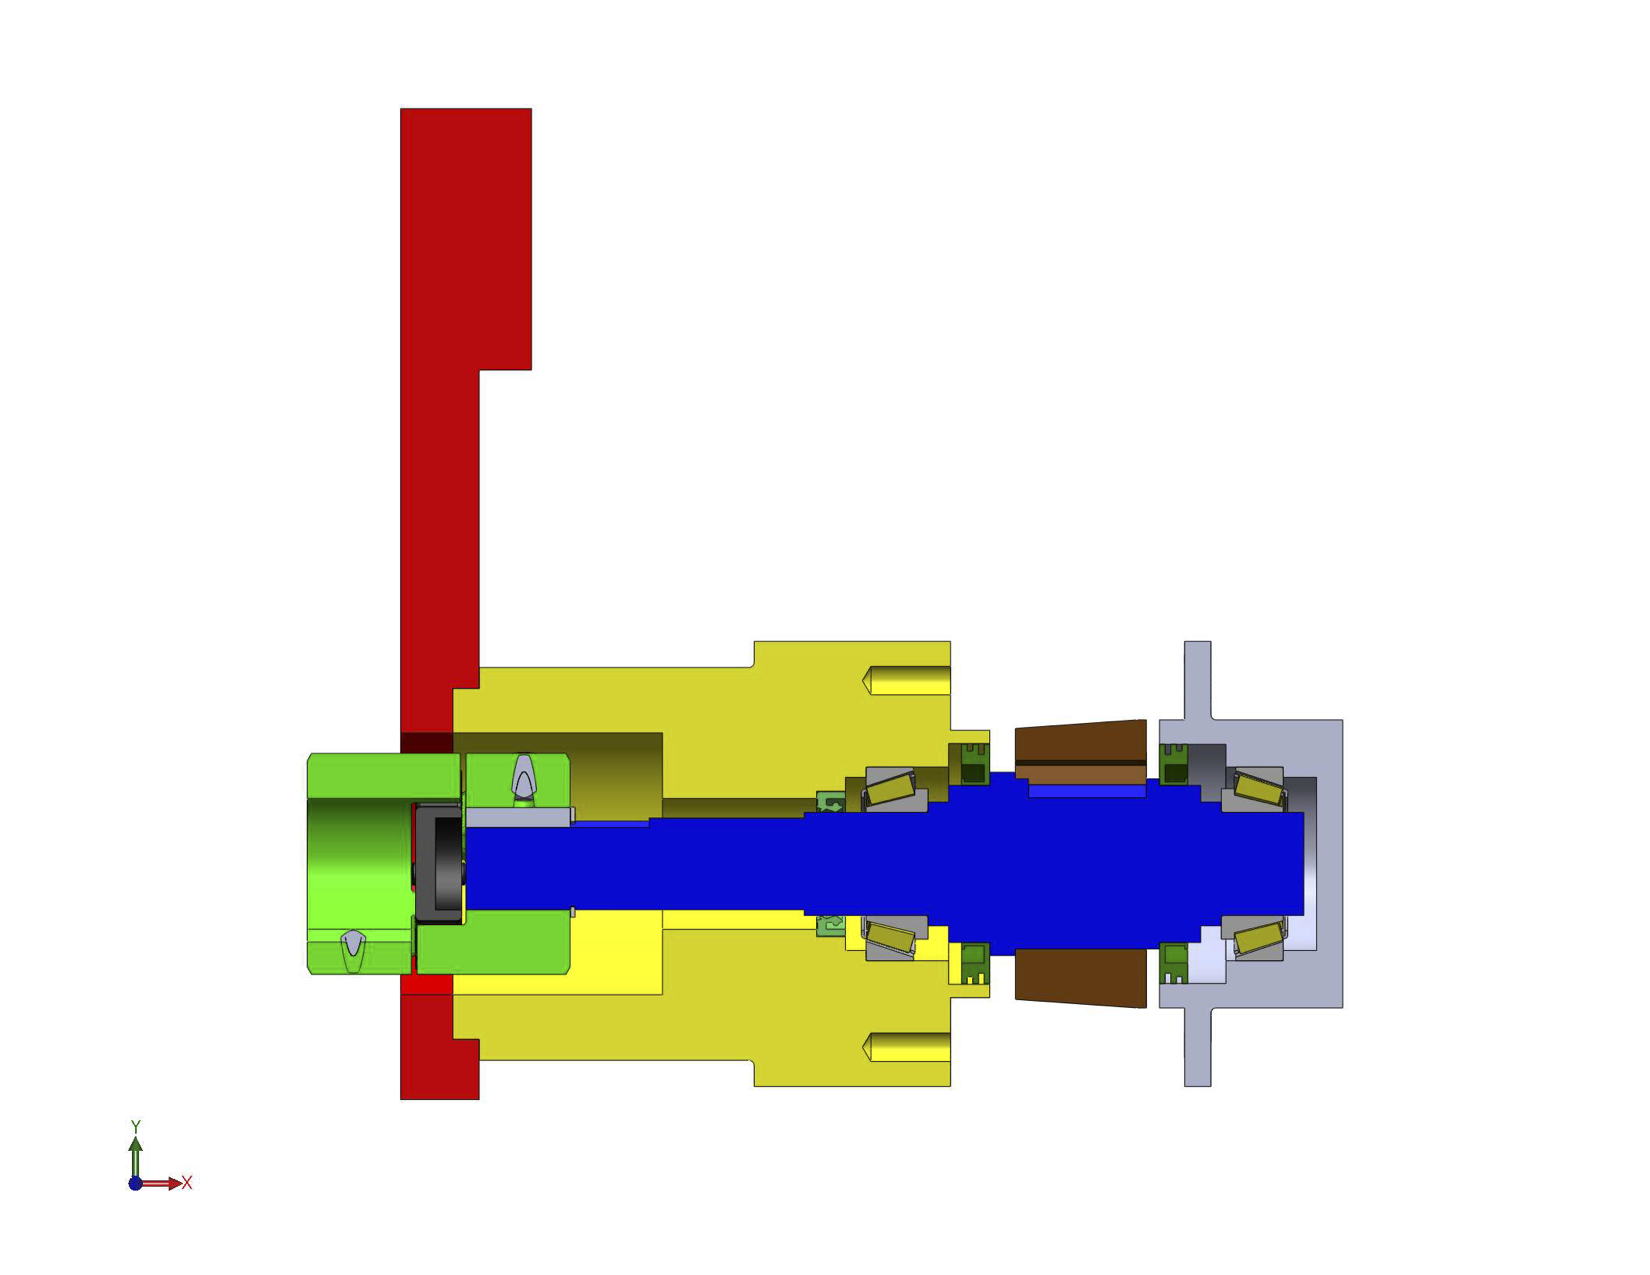
\includegraphics[height=0.3\textheight]{./images/pivot_assembly_drw}
\captionof{figure}[Pivot]{Side view of the the internal and external components of the pivot assembly.}
\label{fig:pivot_assembly_drw}
\end{figure}


\subsubsection{Design Constraints}

The minimum required shaft diameter was calculated using two iterations of DE Goodman shaft design theory. The second iteration took into account more realistic stress concentrations allowing further diameter reduction on the shaft. The shaft layout and loading assumptions are illustrated in Figure~\ref{fig:fb_output_shaft} forces at the ends representing the radial forces applied from the taper roller bearings and the force at the middle being the resultant force of the sprocket determined from the Gates Design IQ software. Bearing calculations were performed according to the procedure outlined in the SKF bearing design manual for taper roller bearings. It is important to note that the free body diagram in Figure~\ref{fig:fb_output_shaft} only represents the radial component of the force from the taper roller bearing, and axial forces not shown were also taken into consideration. Design constraints and requirements are outlined in Table~\ref{tab:drive_const}.  

\begin{figure}[htbp]
\centering
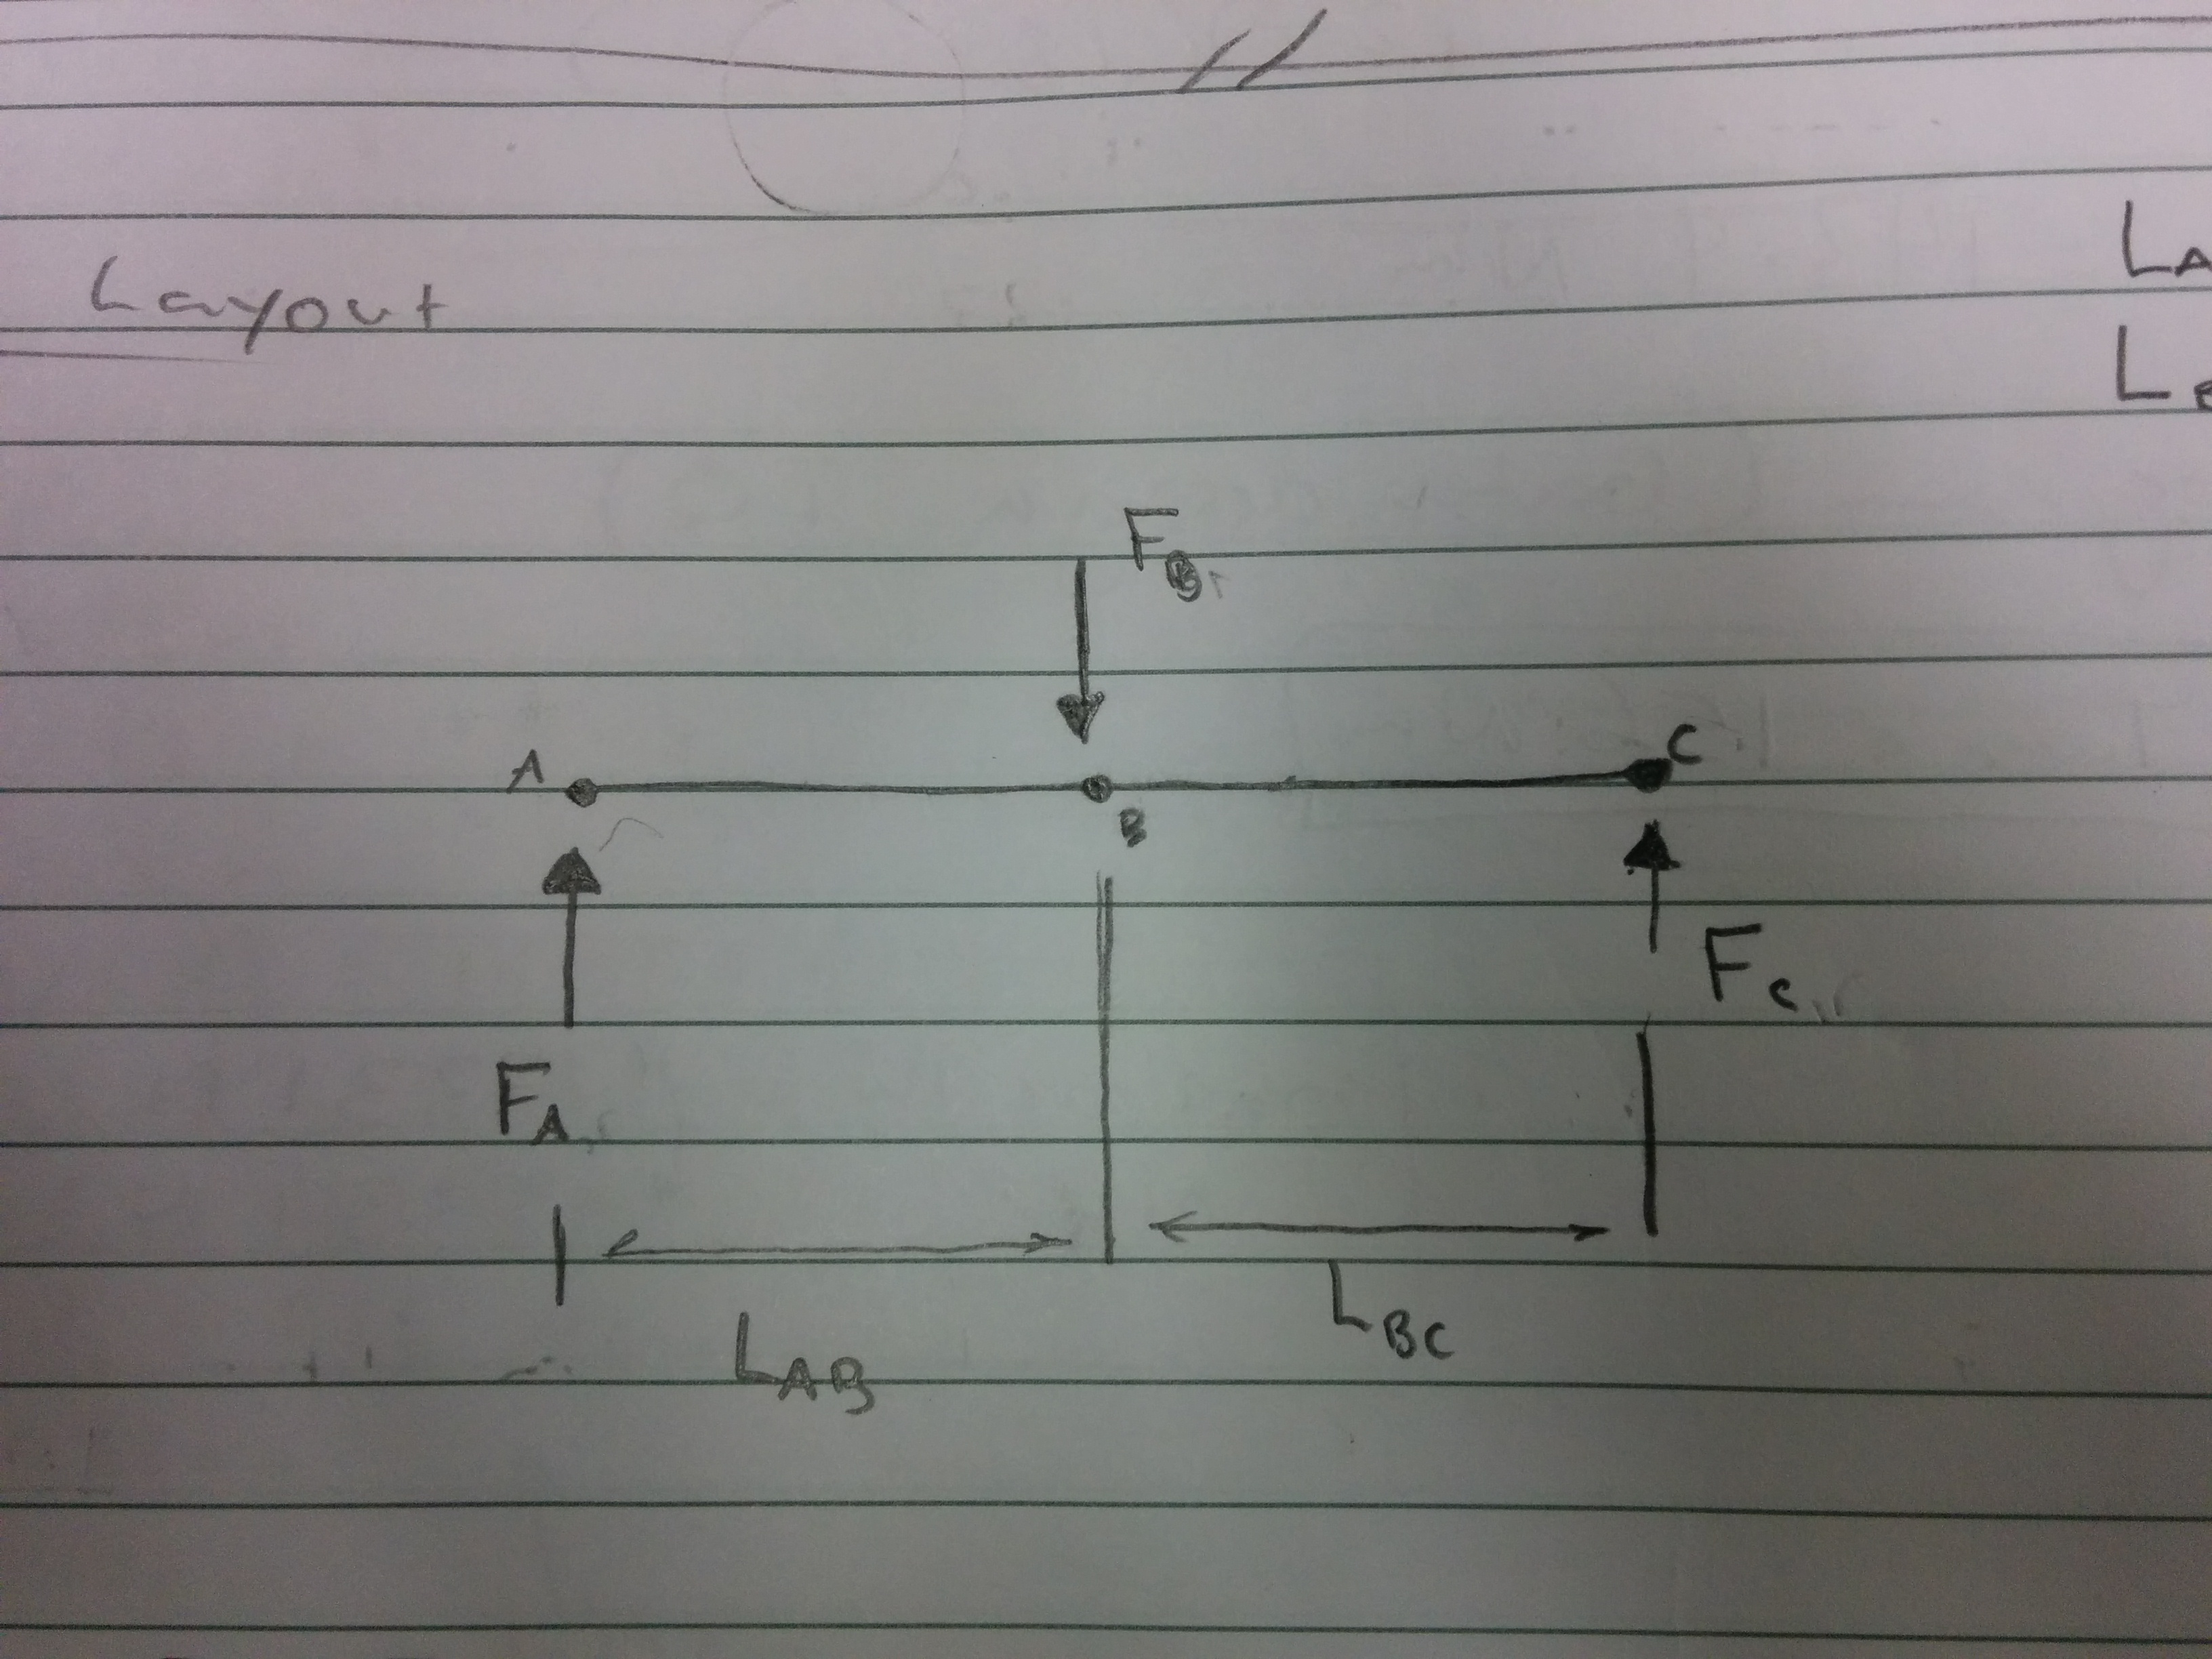
\includegraphics[height=0.3\textheight]{./images/fb_output_shaft}
\captionof{figure}[Pivot]{Drive shaft free body diagram.}
\label{fig:fb_output_shaft}
\end{figure}
\newpage
\begin{table}[htbp]
 \centering
 \caption{Driveshaft Design Constraints and Requirements}
 \begin{tabular}{| llll |} \hline
 Requirement & Value & Unit & Reasoning \\ \hline
 Torque Transmission & 156 & Nm & Maximum torque output of motor \\
 Radial Load & 3331 & N & Radial load applied by sprocket \\ \hline
 \end{tabular}
 \label{tab:drive_const}
 \end{table}

\subsubsection{Functional Requirements}

The pivot is design to create a pivot point for which the drive box can rotate upon and act a rough suspension. But, the pivot is also design to be compact and bear most if not all the stress and strain emitting from the outer drive box during operation. It shouldn't succumb to any plastic bending in either the pivot itself or the bushing and pivot sleeve in the frame insert. Also the limiter should be covered so that no fingers are other body extremities can be pinched during maintenance unless maintenance on the actual limiter. If this is the case, then proper measure should be taken so that no pinching injury happens. The pivot is also design to be modular, as if a section or part of the pivot breaks, replacing the part should be easily managed. 

\subsubsection{Alternate Solution}

Many travel limiter design have been considered. One was comprised as two parts in a circular configuration where the downside of this design was that it was to big to fit in the the instrumentation robot as well as mounting the fixed par of the two would of been a problem. As far as the actual pivot design, there are not many design alternatives besides a eliminating the pivot and the fit the shaft with two coupling that would connect to the drive box. The problem with that design is that it would too complicated and have many issues with respect to strength. 


\subsubsection{Analysis and Design}

The finite element analysis report for all free revisions of the output shaft can be found in APPENDIX A.  The revisions 0 and 2 can be seen in the FIGURE 25 and FIGURE 26 below. In revision 0 the stresses experienced at the end of the output shaft actually exceed the yield strength of the 4340 steel. The changes between the two shaft layouts are significantly different since the first revision was designed to mount radial bearings onto and the final revision now has a taper roller bearing on each end of the sprocket. Seals are also located on both sides of the taper roller bearing to provide a seal. The stresses experienced in the final revision are greatly reduced and do not exceed the yield strength of the material selected. Fillets were also added to reduce the stress concentrations at the shoulders of the different diameters on the shaft. Also, the pivot more than accommodates the bending and stresses coming from the drive box see in FIGURE.

